\chapter{第二章}
\label{sec2}

\section{此小节展示如何引用章节}
\label{sec2.1}

这一段展示下如何引用章节，例如第\ref{sec2}章、第\ref{sec2.1}节。

\section{此小节展示如何插入和引用图片}
\label{sec2.2}

\begin{figure}[!h]
\centering
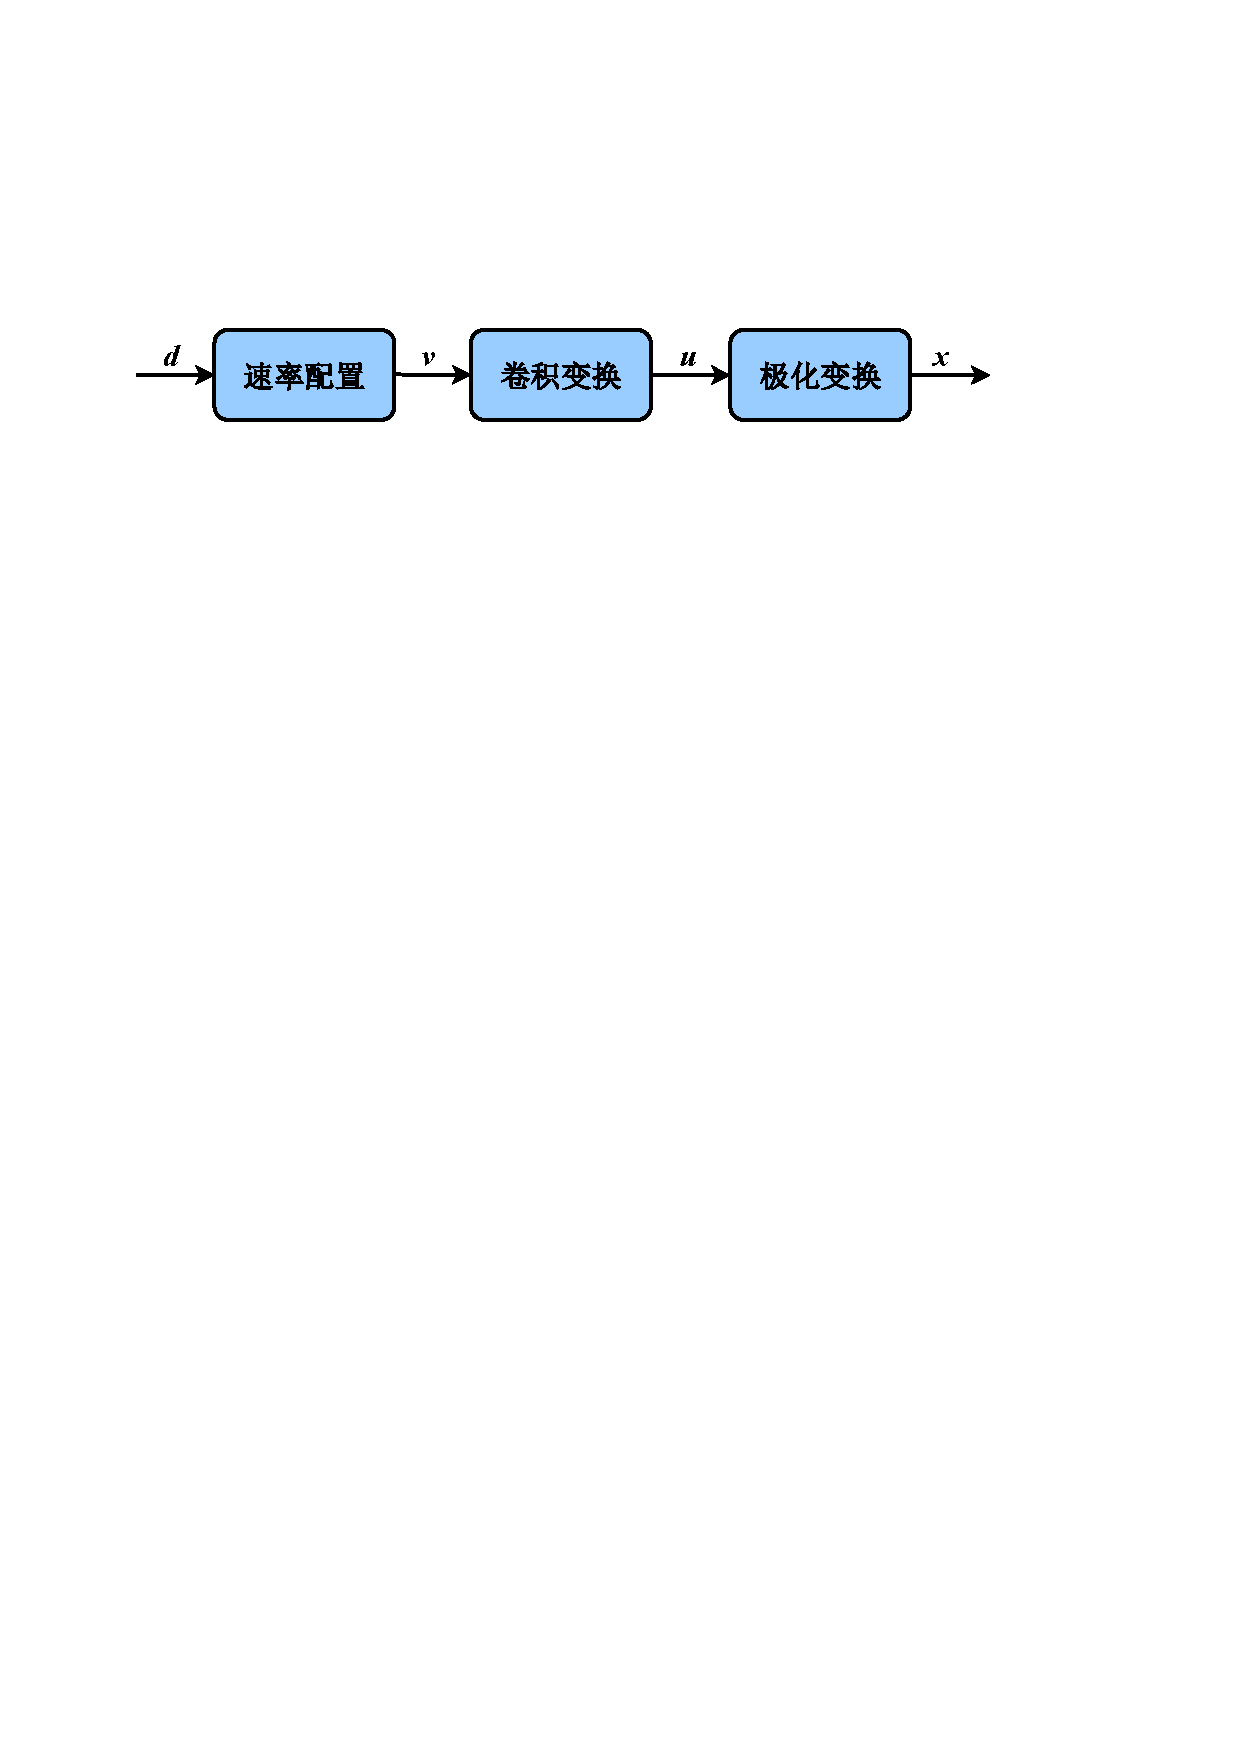
\includegraphics[scale = 0.74]{figures/Chapter 2/2-PAC-Encoder.pdf}
\caption{插入图片的模版}
\label{fig2-1}
\end{figure}

这一段展示下如何引用图片，例如引用图片\ref{fig2-1}。

\section{此小节展示如何插入和引用表格}
\label{sec2.3}

\begin{table}[!h]
\centering
\small
\caption{表格模版}
\label{table2-1}
\resizebox{\columnwidth}{!}{%
\begin{threeparttable}
\begin{tabular}{|cc|c|c|c|c|c|c|}
\hline
\multicolumn{2}{|c|}{（$N$，$R$）} &
  （64，1/2） &
  （128，1/6） &
  （128，1/4） &
  （128，1/2） &
  （128，3/4） &
  （256，1/2） \\ \hline
\multicolumn{2}{|c|}{A}                              & 1040 & 2340  & 22100 & 5460 & 650 & 5330 \\ \hline
\multicolumn{1}{|c|}{\multirow{2}{*}{B}} & $T=4$ & 2048 & 9216 & 1856 & 1280 & 2048 & 1152  \\ \cline{2-8} 
\multicolumn{1}{|c|}{}                          & $T=5$ & 3072 & 9216 & 6656 & 5120 & 2048 & 1152  \\ \hline
\end{tabular}%
\end{threeparttable}
}
\end{table}

这一段展示下如何引用表格，例如引用表格\ref{table2-1}。

\section{此小节展示如何插入和引用公式}
\label{sec2.4}

\begin{flalign}
\label{eq2-1}
\Pr\left({i}\right) = Q(\sqrt {{E}_{1}^i/2} )
\end{flalign}

这一段展示下如何引用公式，例如引用公式\eqref{eq2-1}。

\section{此小节展示如何插入和引用算法表}
\label{sec2.5}

\begin{algorithm}[!h]
\small
\KwIn{$N$、$K$、$\boldsymbol{g}$、${\mathcal{A}}^{\text{temp}}$、$\xi$、目标SNR、$I^{\rm{MC}}$}
\KwOut{${\mathcal{A}}$}
% \KwInti{}
\While{$\xi > K$}{
  将$\boldsymbol{h}\in\mathbb{R}^{1\times N}$中元素初始化为0；\\
  $i = 1$；\\
  \While{$i \leq I^{\rm{MC}}$}{
  利用选定的译码算法在目标SNR对PAC码（$N$，$\xi$，${\mathcal{A}}^{\text{temp}}$，$\boldsymbol{g}$）进行译码；\\
  统计译码结果中的出错位置，并在$\boldsymbol{h}$中相应位置加1；\\
  $i=i+1$；
  }
  搜索$\boldsymbol{h}$中最大值的位置，并将${\mathcal{A}}^{\text{temp}}$中对应位置的索引删除；\\
  计算${\mathcal{A}}^{\text{temp}}$中的索引个数，并用其更新$\xi$；
  
}
${\mathcal{A}}={\mathcal{A}}^{\text{temp}}$；\\
\caption{算法表模板}
\label{alg2-1}
\end{algorithm}

这一段展示下如何引用算法表，例如引用算法表\ref{alg2-1}。


\section{此小节展示如何插入和引用文献}
\label{sec2.6}

这一段展示下如何引用文献，例如在正文中引用文献\incite{Polar-software1} ，或者\cite{Polar-software1} 。
